% Created 2019-08-28 Wed 09:39
% Intended LaTeX compiler: pdflatex
\documentclass[11pt]{article}
\usepackage[utf8]{inputenc}
\usepackage{lmodern}
\usepackage[T1]{fontenc}
\usepackage{fixltx2e}
\usepackage{graphicx}
\usepackage{longtable}
\usepackage{float}
\usepackage{wrapfig}
\usepackage{rotating}
\usepackage[normalem]{ulem}
\usepackage{amsmath}
\usepackage{textcomp}
\usepackage{marvosym}
\usepackage{wasysym}
\usepackage{amssymb}
\usepackage{amsmath}
\usepackage[theorems, skins]{tcolorbox}
\usepackage[version=3]{mhchem}
\usepackage[numbers,super,sort&compress]{natbib}
\usepackage{natmove}
\usepackage{url}
\usepackage{minted}
\usepackage{underscore}
\usepackage[linktocpage,pdfstartview=FitH,colorlinks,
linkcolor=blue,anchorcolor=blue,
citecolor=blue,filecolor=blue,menucolor=blue,urlcolor=blue]{hyperref}
\usepackage{attachfile}
\usepackage[left=1in, right=1in, top=1in, bottom=1in, nohead]{geometry}
\geometry{letterpaper}
\usepackage{outline}
\usepackage{amsmath}
\usepackage{graphicx}
\usepackage{epstopdf}
\usepackage{siunitx}
\usepackage{bm}
\usepackage{parskip}
\usepackage[version=3]{mhchem}
\usepackage[labelfont=bf]{caption}
\usepackage{hyperref}
\hypersetup{colorlinks=true,urlcolor=blue}
\setlength{\headheight}{15.2pt}
\usepackage{fancyhdr}
\pagestyle{fancy}
\fancyhf{}
\renewcommand{\headrulewidth}{0.5pt}
\renewcommand{\footrulewidth}{0.5pt}
\lfoot{\today}
\cfoot{\copyright\ 2019 W.\ F.\ Schneider}
\rfoot{\thepage}
\lhead{\em{Computational Chemistry}}
\rhead{ND CBE 60547}
\def\dbar{{\mathchar'26\mkern-12mu d}}
\setcounter{secnumdepth}{3}
\author{William F. Schneider}
\date{\today}
\title{Lecture Notes for CBE 60547}
\begin{document}

\setcounter{tocdepth}{2}
\tableofcontents

\begin{OPTIONS}
\end{OPTIONS}

\section{Introduction}
\label{sec:org5b780be}
\subsection{What do we care about?}
\label{sec:org16c6e04}

Things chemistry/materials-related:

\begin{itemize}
\item What are the properties of atoms?
\item What molecules do they make?  What other substances do they make?
\item What are the shapes of those molecules?  Structures of those solids?  Properties of them?
\item How do those substances react with each other?
\item What are the energies of those reactions?
\item What are the rates of those reactions?
\item What is the strongest substance?
\item How do we make a substance to do\ldots{}.?
\item add your own questions\ldots{}.
\end{itemize}

Things that relate to the \emph{chemical} properties of substances.

\subsection{How are we going to figure these out?  With only a computer?}
\label{sec:orgf023153}
\begin{description}
\item[{1926}] Erwin Schr\"{o}dinger equation: \(\hat{H}\Psi=E\Psi\)
\item[{1929}] Paul Dirac, British physicist
\end{description}

\begin{quote}
The fundamental laws necessary for the mathematical treatment of a
large part of physics and the whole of chemistry are thus \emph{completely
known}, and the difficulty lies only in the fact that application of
these laws leads to equations that are \emph{too complex to be solved}.

It therefore becomes desirable that \emph{approximate practical methods} of
applying quantum mechanics should be developed, which can lead to an
explanation of the main features of complex atomic systems without
too much computation.
\end{quote}

\begin{description}
\item[{1930's-1950's}] Elaboration, analytical applications

\item[{1950's}] Computers start to appear for technical applications

\item[{1960's}] Density functional theory emerges.

\item[{1960's-1970's}] Numerical solutions of Schr\"{o}dinger equation for atoms/molecules---expert users

\item[{1980's}] ``Supercomputer'' era---routine use of computational chemistry software becomes possible
\end{description}
\begin{figure}[htbp]
\centering
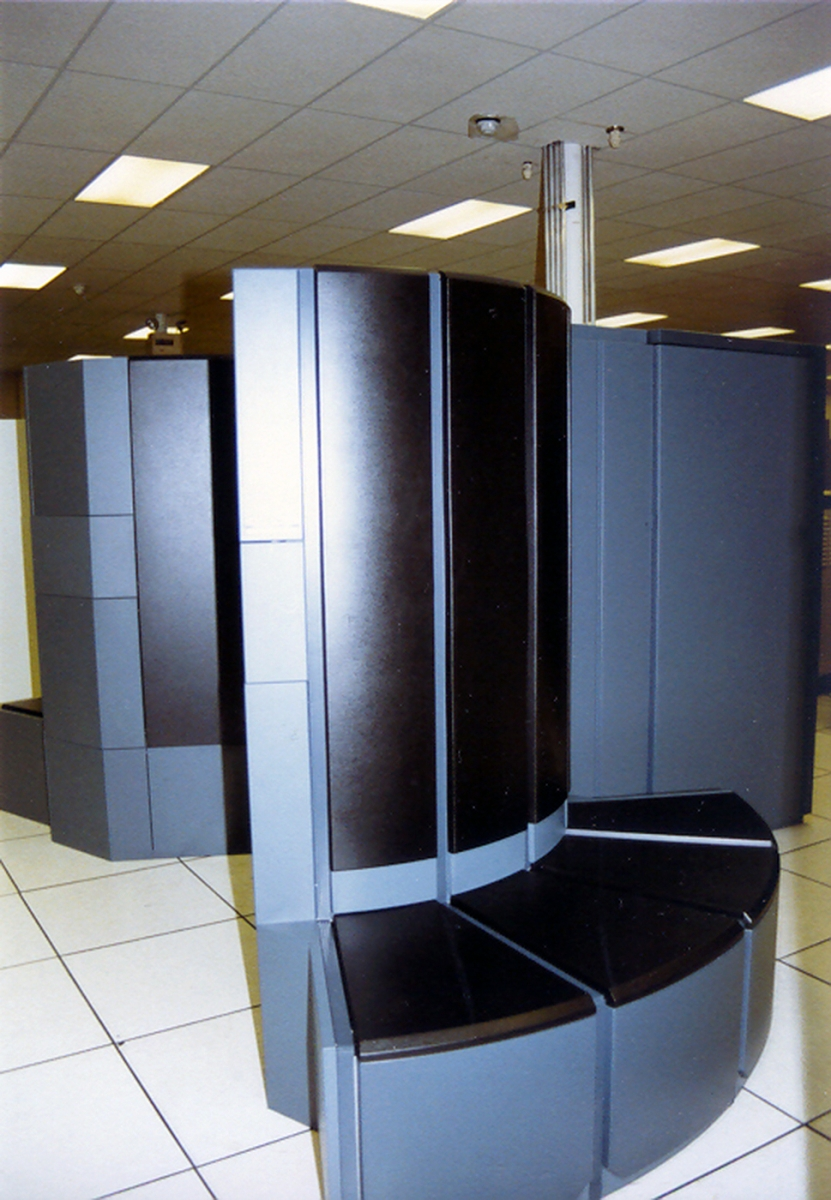
\includegraphics[width=0.2\textwidth]{./Images/CrayYMPb.jpg}
\caption{Ohio State Cray Y-MP supercomputer, ca. 1989.  World's fastest computer at the time.  333 MFlop top speed, 512 Mb RAM}
\end{figure}

\begin{description}
\item[{1990's}] ``Chemical accuracy'' era---very precise solutions routinely available, for a cost!  See \href{./Resources/1994\_WFS\_JPC.pdf}{Schneider, \emph{JPC} \textbf{1994}}.

\item[{1990's}] Density functional theory (DFT) allows applications to solids/surfaces/liquids to become common. See \href{./Resources/1998\_Hass\_Science.pdf}{Hass, \emph{Science}, \textbf{1998}}

\item[{1990's}] Visualization moves to the desktop

\item[{2000's}] Computational ``screening,'' materials discovery (\href{http://www.crc.nd.edu/\~wschnei1/courses/CBE\_547/Resources/2010\_Gurkan\_JPCL.pdf}{Gurkan, \emph{J. Phys. Chem. Lett.}, \textbf{2010}}), materials genome (\url{https://materialsproject.org/}).

\item[{Today}] Computational chemistry widely integrated into all aspects of chemical, materials, biological research
\end{description}

\texttt{Computational chemistry} is now so vast it is impossible to cover everything completely.  We limit ourselves to quantum-mechanics-based calculations.

\subsection{Our goals}
\label{sec:org413b556}
\begin{enumerate}
\item Understand when it is appropriate to use quantum-mechanics methods.
\item Be able to state the basic theoretical, mathematical, and numerical concepts behind quantum mechanical ``wavefunction theory'' (WFT) and ``density functional theory,'' (DFT) calculations.
\item Understand the terminology and practical issues associated with doing quantum chemical simulations.
\item Get hands-on experience with these concepts using popular computational tools of today, including GAMESS for molecular systems and Vasp for condensed phase systems.
\item Learn how to set up, execute, and analyze results in a modern, Python notebook environment.
\item Learn how to apply the results of quantum chemical simulations to calculate things you care about.
\item Demonstrate an ability to formulate a problem and apply QM  methods to it.
\item Develop the skills to understand a literature paper in the area.
\end{enumerate}

\subsection{Reading resources}
\label{sec:org629495e}
\begin{itemize}
\item These notes
\item Chris Cramer, \emph{Essentials of Computational Chemistry}, Wiley, 2004
\item Martin,
\item Sholl and Steckel, \emph{Density Functional Theory: A Practical Introduction}, Wiley, 2009
\item Kitchin book, \url{http://kitchingroup.cheme.cmu.edu/dft-book/}
\end{itemize}

\subsection{Software tools}
\label{sec:orgddc0e3b}
\subsubsection{Notebooks}
\label{sec:org89e3c37}
\begin{itemize}
\item org-mode
\item jupyter/ipython
\end{itemize}

\subsubsection{Molecular methods}
\label{sec:org8ed5b8c}
\begin{itemize}
\item Avogadro environment \url{http://avogadro.cc/wiki/Main\_Page}
\item GAMESS code \url{http://www.msg.ameslab.gov/GAMESS/GAMESS.html}
\end{itemize}

\subsubsection{Supercell methods}
\label{sec:org62ae2f5}
\begin{itemize}
\item ASE environment \url{https://wiki.fysik.dtu.dk/ase/}
\item Vasp code \url{http://www.vasp.at/}
\end{itemize}

\subsubsection{Great for getting started}
\label{sec:org239ad3c}
\begin{itemize}
\item Webmo \url{http://www.webmo.net/}
\end{itemize}
\newpage

\section{Refresher on Quantum Mechanics}
\label{sec:org32044bb}
\subsection{Why quantum mechanics?}
\label{sec:orgccecf22}
Want to describe ``mechanics'' (equations of motion) of atomic-scale things, like electrons in atoms and molecules

Why? These ultimately determine the energy, the shape, and all the properties of matter.

\emph{de Broglie wavelength} (1924)
\begin{equation}
\lambda  = h/p = h/mv
\end{equation}
\begin{equation}
h  = \SI{6.626e-34}{J.s} \text{(Planck's constant)}
\end{equation}

\begin{center}
\begin{tabular}{lll}
\hline
 & Car & Electron\\
\hline
mass \(m\) & \SI{1000}{kg} & \SI{9.1e-31}{kg}\\
velocity \(v\) & \SI{100}{km/hr} & \SI{0.01}{c}\\
 & typical value on the highway & typical value in an atom\\
momentum \(p\) & \SI{2.8e-4}{kg.m/s} & \SI{2.7e-24}{kg.m/s}\\
wavelength \(\lambda\) & \SI{2.4e-38}{m} & \SI{2.4e-10}{m}\\
 & too small to detect.  Classical! & Comparable to size of an atom.\\
 &  & \emph{Must} treat with QM!\\
\hline
\end{tabular}
\end{center}

How to describe wave properties of an electron?  Schr\"{o}dinger equation (1926)

\begin{center}
Kinetic energy + Potential energy = Total Energy
\end{center}

Expressed as differential equation (Single particle, non-relativistic):
\begin{equation}
-\frac{\hbar^2}{2m}\nabla^2 \Psi(\mathbf{r},t) + V(\mathbf{r},t)  \Psi(\mathbf{r},t) = -i \hbar \frac{\partial}{\partial t}  \Psi(\mathbf{r},t)
\end{equation}

If the potential \(V\) is time-invariant, can use separation of variables to
show that the steady-state, time-independent solutions are characterized by an
energy \(E\) and described by:
\begin{eqnarray}
-\frac{\hbar^2}{2m}\nabla^2 \psi(\mathbf{r}) + V(\mathbf{r})  \psi(\mathbf{r}) = E \psi(\mathbf{r}) \\
\Psi(\mathbf{r},t) = \psi(\mathbf{r})e^{-iEt/\hbar}
\end{eqnarray}

\subsection{Postulates of non-relativistic quantum mechanics}
\label{sec:orgdcac91a}
\begin{table} 
\begin{center}
    \caption{\large{Postulates of Non-relativistic Quantum Mechanics}}
   \begin{description}
    \item[Postulate 1:] {{\bf The physical state of a system is completely described by
        its wavefunction $\Psi$.}  In general, $\Psi$ is a complex function of the spatial
      coordinates and time.  $\Psi$ is required to be:}
    \begin{outline}
      \item{Single-valued}
      \item {continuous and twice differentiable}
      \item {square-integrable ($\int \Psi^*\Psi d\tau$ is defined over all finite domains)}
      \item {For bound systems, $\Psi$ can always be normalized such that $\int \Psi^*\Psi d\tau=1$}
    \end{outline}

  \item[Postulate 2:]  To every physical observable quantity $M$ there corresponds a
    Hermitian operator $\hat{M}$.  {\bf The only observable values of $M$ are the
      eignevalues of $\hat{M}$.}
    \begin{center}
    \begin{tabular}[h]{ccc}
      \hline
{\bf Physical quantity} & {\bf Operator} & {\bf Expression} \\
\hline
Position $x,y,z$ & $\hat{x},\hat{y},\hat{z}$ & $x\cdot, y\cdot, z\cdot$ \\ \\
Linear momentum $p_x, \ldots$ & $\hat{p}_x,\ldots $ & $\displaystyle -i\hbar\frac{\partial}{\partial
  x},\ldots $\\
Angular momentum $l_x, \ldots$ & $\hat{p}_x,\ldots $ & $\displaystyle -i\hbar \left
  (y\frac{\partial}{\partial z}-z\frac{\partial}{\partial y}\right ), \ldots $ \\
Kinetic energy $T$ & $\hat{T}$ & $\displaystyle -\frac{\hbar^2}{2m}\nabla^2$ \\
Potential energy $V$ & $\hat{V}$ & $V({\bf r},t)$ \\
Total energy $E$ & $\hat{H}$ & $\displaystyle -\frac{\hbar^2}{2m}\nabla^2+V({\bf r},t)$\\ \\
\hline
    \end{tabular}
  \end{center}
    \item[Postulate 3:] {If a particular observable $M$ is measured many times on many
      identical systems is a state $\Psi$, the average resuts with be the expectation
      value of the operator $\hat{M}$:
      \begin{equation*}
        \langle M \rangle = \int \Psi^* (\hat{M}\Psi)d{\bf\tau}
      \end{equation*}}
    \item[Postulate 4:] {The energy-invariant states of a system are solutions of the equation
        \begin{eqnarray*}
          \hat{H}\Psi({\bf r},t) & = & i\hbar\frac{\partial}{\partial t}\Psi({\bf r},t) \\
          \hat{H} & = & \hat{T}+\hat{V}
        \end{eqnarray*}
      The time-independent, stationary states of the system are solutions to the equation
      \begin{equation*}
        \hat{H}\Psi({\bf r}) = E\Psi(\bf{r})
      \end{equation*}
}
    \item[Postulate 5:] (The {\bf uncertainty principle}.)  Operators that do not commute
      $(\hat{A}(\hat{B}\Psi)\neq\hat{B}(\hat{A}\Psi))$ are called {\em conjugate}.
      Conjugate observables cannot be determined simultaneously to arbitrary accuracy.
      For example, the standard deviation in the measured positions and momenta of
      particles all described by the same $\Psi$ must satisfy $\Delta x\Delta p_x \geq \hbar/2$.
    \end{description}
\end{center}
\end{table}

\subsection{Notes on constants and units}
\label{sec:org3ad47b3}
Resource on physical constants: \url{http://physics.nist.gov/cuu/Constants/}
Resource for unit conversions: \url{http://www.digitaldutch.com/unitconverter/}

Unit converter available in Calc mode of Gnu emacs \textbf{highly recommended}

\begin{table}[htbp]
\caption{Atomic units common for quantum mechanical calculations (see \url{http://en.wikipedia.org/wiki/Atomic\_units})}
\centering
\begin{tabular}{llll}
\hline
 & Atomic unit & SI unit & Common unit\\
\hline
Charge & \(e = 1\) & \SI{1.6021e-19}{C} & \\
Length & \(a_0 = 1\) (bohr) & \SI{5.29177e-11}{m} & \SI{0.529177}{\AA}\\
Mass & \(m_e = 1\) & \SI{9.10938e-31}{kg} & \\
Angular momentum & \(\hbar = 1\) & \SI{1.054572e-34}{J.s} & \\
Energy & \(E_h = 1\) (hartree) & \SI{4.359744e-18}{J} & \SI{27.2114}{eV}\\
Electrostatic force & \(1/(4\pi\epsilon_0) = 1\) & \SI{8.987552e-9}{N.m^2/C^2} & \\
Boltzmann constant &  & \SI{1.38065e-23}{J\per K} & \SI{8.61733e-5}{eV/K}\\
\hline
\end{tabular}
\end{table}


\begin{center}
Energy units
1 eV = \SI{1.60218e-19}{J} = \SI{96.485}{kJ/mol} = \SI{8065.5}\{cm\(^{\text{-1}}\)\} = \SI{11064}{K.k_B}
\end{center}

\subsection{Example: Energy states of a particle in a box}
\label{sec:org59e874a}

System defined by potential experienced by particle:

\(V(\mathbf{r}) = 0,\qquad 0 < x,y,z < L\)

\(V(\mathbf{r}) = \infty,\qquad x,y,z \leq 0,\ x,y,z \geq L\)

\begin{center}
\begin{center}
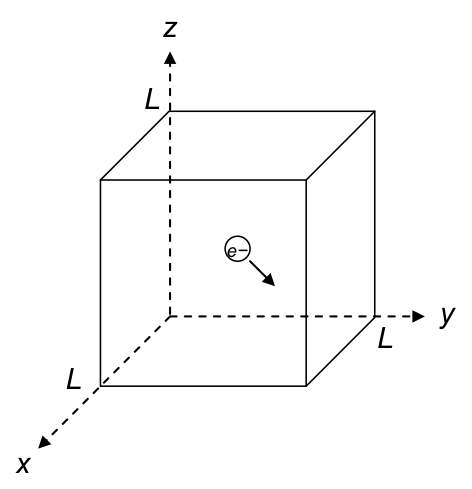
\includegraphics[width=0.3\textwidth]{./Images/Cube.png}
\end{center}
\end{center}

3D box \(\rightarrow\) 3 degrees of freedom/coordinates

\textbf{Schr\"{o}dinger equation}
\begin{equation}
-\frac{\hbar^2}{2m_e} \left ( \frac{\partial^2 }{\partial x^2} + \frac{\partial^2 }{\partial y^2} + \frac{\partial^2 }{\partial z^2} \right ) \psi(x,y,z) = E \psi(x,y,z)
\end{equation}
\begin{equation}
\psi(x,y,z) = 0, \quad x,y,z \leq 0,\ x,y,z \geq L
\end{equation}

A second-order, linear, partial differential equation.  Boundary value problem. Solve by separation of variables.  Postulate \(\psi(x,y,z) = X(x)Y(y)Z(z)\). Substituting and rearrange to get

\begin{equation}
-\frac{\hbar^2}{2m_e} \left (\frac{1}{X(x)}\frac{\partial^2 X(x)}{\partial x^2} + \frac{1}{Y(y)}\frac{\partial^2 Y(y)}{\partial y^2} + \frac{1}{Z(z)}\frac{\partial^2 Z(z)}{\partial z^2} \right ) = E \qquad 0 < x,y,z <L
\end{equation}

ftn x + ftn y + ftn z = constant \(\rightarrow\) each term must be constant.

\textbf{Equation for each dimension}
\begin{equation}
-\frac{\hbar^2}{2m_e}\frac{\partial^2 X(x)}{\partial x^2} = E_x X(x), \qquad X(0)=X(L) = 0
\end{equation}

Seek function that twice differentiated returns itself and satisfies boundary conditions.
\begin{equation}
X(x) = \sin\frac{n_x\pi x}{L},\qquad n_x = 1,2,3,\ldots
\end{equation}

\begin{equation}
E_{n_x} = \frac{n_x^2\pi^2\hbar^2}{2 m_e L^2}
\end{equation}

Solutions called \emph{eigenfunctions} (or \emph{wavefunctions}) and \emph{eigenvalues}.  Characterized
by \emph{quantum numbers}, one for each degree of freedom.  These (and all QM) solutions have certain
special properties, including that they are orthonormal and form a complete set.

\textbf{Normalization}

Seek a constant such that the inner eigenfunction product is unity.
\begin{eqnarray}
C^2 \int_0^L \sin^2 \frac{n_x\pi x}{L} dx = C^2 L/2 = 1 \rightarrow C=\pm\sqrt{\frac{2}{L}}\\
X(x) = \pm\sqrt{\frac{2}{L}}\sin\frac{n_x\pi x}{L},\qquad n_x = 1,2,3,\ldots
\end{eqnarray}

\textbf{Orthonormal}
\begin{equation}
\langle X_{n_x} | X_{n^\prime_x} \rangle = \delta_{n_{x},n_x^\prime}\qquad
\text{Dirac notation}
\end{equation}

\begin{center}
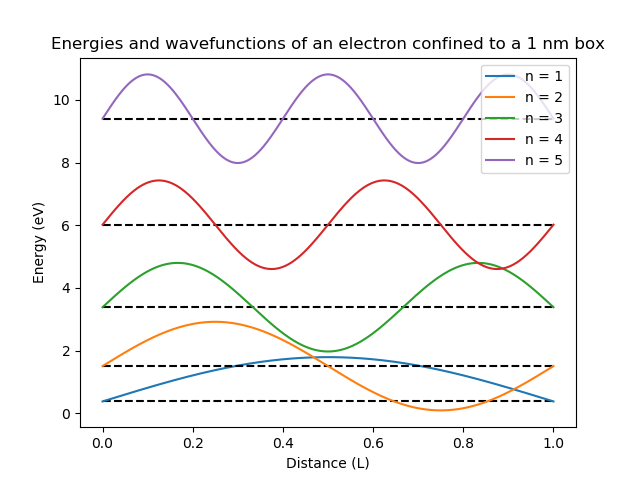
\includegraphics[width=0.75\textwidth]{./Images/1DPIAB.png}
\end{center}

\begin{itemize}
\item Energy increase with number of \emph{nodes}.

\item \(E\propto n^2, \Delta E \propto n, \Delta E/E \propto 1/n\).  \emph{Relative} spacing decreases with \(n\).

\item Is this real?  See \href{http://dx.doi.org/10.1021/jp053496l}{Ho, \emph{J. Phys. Chem. B} \textbf{2005}, \emph{109}, 20657}.
\end{itemize}

\textbf{Three-dimensional solutions}
\begin{equation}
\psi(x,y,z) = X(x)Y(y)Z(z) = \left ( \frac{2}{L} \right )^{3/2} \sin\frac{n_x\pi x}{L}\sin\frac{n_y\pi y}{L}\sin\frac{n_z\pi z}{L},\qquad n_{x},n_{y},n_{z}=1,2,3,\ldots
\end{equation}
\begin{equation}
\label{eq:2}
E = E_{x}+E_{y}+E_{z}=\frac{(n_{x}^{2}+n_{y}^{2}+n_{z}^{2}) \pi^{2}\hbar^{2}}{2 m L^{2}}
\end{equation}

\begin{center}
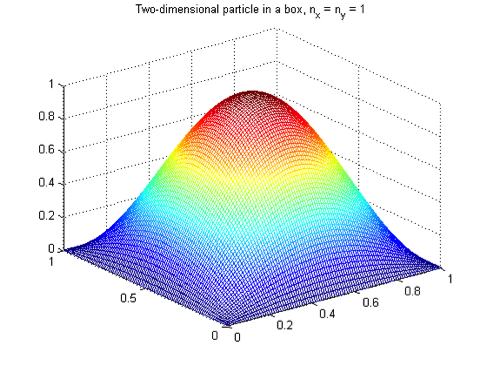
\includegraphics[width=0.5\textwidth]{./Images/2DSine1.png}
\end{center}
\begin{center}
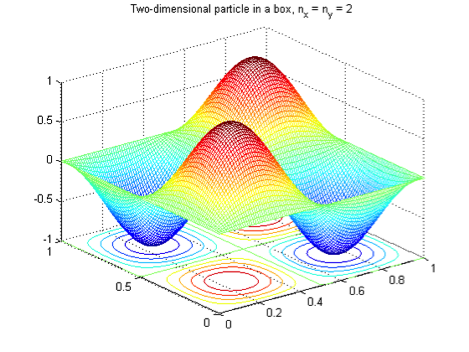
\includegraphics[width=0.5\textwidth]{./Images/2DSine2.png}
\end{center}


\begin{figure}[htbp]
\centering
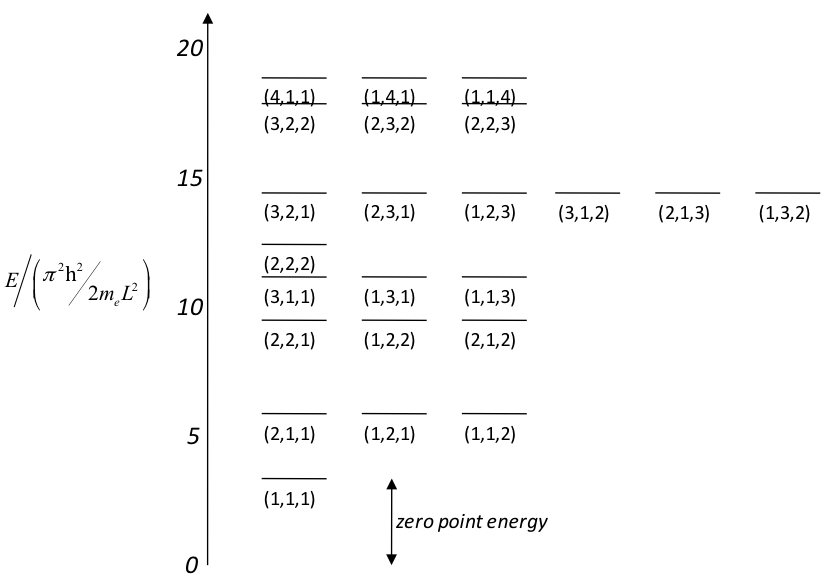
\includegraphics[width=.9\linewidth]{./Images/3DEnergyStates.png}
\caption{Energy sates of 3D Particle in a box}
\end{figure}

Properties of solutions:
\begin{itemize}
\item Symmetry of system introduces degeneracy in solutions
\item Energy depends on volume \(\rightarrow\) pressure!
\end{itemize}

\newpage

\section{Hydrogen atom}
\label{sec:org511e4fa}
\subsection{Hydrogen atom solutions}
\label{sec:org2436e20}
\subsection{Variational principle}
\label{sec:orgb3721f2}
\subsection{Basis functions}
\label{sec:orgf8be288}
\subsection{Secular equations}
\label{sec:org4052a1e}
\subsection{Spin}
\label{sec:org44bf568}
\newpage

\section{(Two is too) many electrons}
\label{sec:orgb5c4224}
\href{./Resources/2009\_Greeley\_JPCC.pdf}{Greeley, \emph{JPCC}, \textbf{2009}}** What's the problem?
Helium: next (after hydrogen) simplest atom

In a sense, we ``know'' the answer\ldots \(1s^2\).  But is this same \(1s\) as H?  No!  Different nuclear charge, interactions between the two electrons.  This is an approximation and a very convenient shorthand!

\subsubsection{Schr\"{o}dinger equation for He}
\label{sec:org004ab59}
Wavefunction \(\Psi(\mathbf{r}_1,\mathbf{r}_2)\), atom energy \(E\).

Define 1-electron operator for each electron, in atomic units.  Include kinetic energy of electron and its attraction to nucleus of charge \(Z=2\):
\[\hat{h}_i = -\frac{1}{2}\nabla^2_i -\frac{Z}{|\mathbf{r}_i|}\]
Looks similar to hydrogen atom.

BUT, electrons also repel.  Total Schr\"{o}dinger equation for He:
\[\left\{\hat{h}_1 + \hat{h}_2 + \frac{1}{|\mathbf{r}_2 - \mathbf{r}_1|\right\}\Psi(\mathbf{r}_1,\mathbf{r}_2) = E\Psi(\mathbf{r}_1,\mathbf{r}_2) }\]
Last term accounts for electron-electron electrostatic repulsion.  Makes problem non-separable and really hard to solve. (How many solutions are there?)

Generalize to \(n\)-electron atom, in atomic units:
\begin{eqnarray}
\hat{H} & = & \sum_i \hat{h}_i + \sum_{j>i+1}\frac{1}{|\mathbf{r}_j - \mathbf{r}_i|} \\
\hat{H} \Psi(\mathbf{r}_1,\ldots,\mathbf{r}_n) & = & E\Psi(\mathbf{r}_1,\ldots,\mathbf{r}_n) \end{eqnarray}

First summation over all electrons, second gets all electron pairs.

Solutions are many-dimensional functions of the coordinates of all the electrons.  Cannot solve this analytically, although approaches exist (eg quantum Monte Carlo) that can in principle get very close.  Thankfully, though, we can make approximations that work out really well.  We'll look at three historically important ones.

\subsection{The Hartree atom}
\label{sec:org27b7082}
Simplest approach is to approximate \(\Psi\). Douglas Hartree (1897-1958) writes:
\[ \Psi(\mathbf{r}_1,\mathbf{r}_2) \approx \psi_1(\mathbf{r}_1)\cdot \psi_n(\mathbf{r}_n)\]
So-called Hartree product.  Can't be right.  It gives the probability of two electrons being in the same place as some number \(> 0\)!  Neglects \emph{electron correlation}.  How to apply?

\begin{enumerate}
\item Apply variational principle: What's the best possible set of \(\psi_i\)?  We'll say best are the set that give the lowest expectation value of energy.
\begin{eqnarray}
\langle E \rangle & = & \langle \Psi | \hat{H} | \Psi \rangle \\
\frac{ \delta \langle E \rangle}{\delta \psi_i} &= &0, \forall i
\end{eqnarray}
\item Lagrange multipliers to impose orthonormality constraint on \(\psi_i\):
\begin{eqnarray}
  \langle \psi_i | \psi_j \rangle &=& \delta_{ij} \\
   L & = & \langle E \rangle - \sum_{i,j}\epsilon_{ij}\left ( \langle \psi_i | \psi_j \rangle - \delta_{ij} \right ) \\
 \delta L &=& 0
 \end{eqnarray}
\item Coupled, one-electron Hartree eigenvalue equations for energy-optimal \(\psi_i\):
\begin{eqnarray}
 \left \{ \hat{h}_i + \hat{v}^{\text{Hartree}}_i \right \} \psi_i(\mathbf{r}_1) &=&         \epsilon_i      \psi_i(\mathbf{r}_1) \\
   \hat{v}^{\text{Hartree}}_i(\mathbf{r}_i) & =& \sum_{j\ne i} \int \left | \psi_j(\mathbf{r}_2) \right      |^2\frac{1}{|\mathbf{r}_2-\mathbf{r}_1|}d\mathbf{r}_2
       \end{eqnarray}
\end{enumerate}
Have to solve this for all \emph{n} electrons of an atom/molecule. ``Hartree potential'' represents Coulomb repulsion between electron \emph{i} and all other electrons, \emph{averaged} over position of those electrons.  Always positive.  This is a \emph{mean field} approximation.  Note appearance of ``one electron'' energies, \(\epsilon_i\), kinetic energy plus repulsion of electron with all others.  Total energy is sum of these \(\epsilon_i\) corrected to avoid overcounting repulsions:
\[ \langle E \rangle = \sum_i \epsilon_i - \frac{1}{2}\sum_i \langle \psi_i| \hat{v}^{\text{Hartree}}_i|\psi_i\rangle \]

Presents an obvious difficulty.  If we don't know \(\psi_j\) ahead of time, how can we even construct Hartree equations, let alone solve them?  Hartree offered a numerical solution, in the 1930's, called the \textbf{\emph{self-consistent field} (SCF) approach}:
\begin{enumerate}
\item Guess an initial set of \(\psi_i\), one for each electron (he did this on a grid, and
jumping ahead a bit, allowed each \(\psi_i\) to represent two electrons)
\item Construct Hartree potential for each \(\psi_i\)
\item Solve the \(n\) differential equations for \(n\) new \(\psi_i\)
\item Compare new to old \(\psi_i\)
\item If the same within a desired tolerance, you are done!
\item If not, return to step 2, using new \(\psi_i\), and repeat.
\end{enumerate}

Hartree's father did this by hand for all the atoms of the periodic table, tabulating wavefunctions and energies for all the electrons in each.  For instance, for He, he'd solve one equation, self-consistently, to get one \(\psi_1\), and then combine to get \(\Psi(1,2) = \psi_1(1)\alpha(1)\psi_1(2)\beta_2\).  Tedious!  Qualitatively great, quantitatively not so hot.  Mean-field approximation just not so hot.

Nonetheless, basic idea of representing many-body wavefunction in terms of ``orbitals,'' of setting up orbital equations, and solving using a self-consistent procedure, remain today at the heart of virtually all electronic structure calculations.  Hurrah Hartree!
\subsection{The Pauli principle}
\label{sec:orgdb01f61}
One big conceptual short-coming of the Hartree model is that it treats the electrons as if they were distinguishable. QM says electrons are indistinguishable.  Furthermore, they have a quantized angular momentum, called a spin, that is either up or down, making them fermions.  
\newpage
\begin{quote}
\textbf{Pauli principle}: The wavefunction of a multi-particle fermion system must be anti-symmetric to coordinate exchange.
\end{quote}
\[\Psi(\bm{x}_1, \bm{x}_2) = -\Psi(\bm{x}_2, \bm{x}_1) \]

Here the coordinate \textbf{x} includes both the position and the spin (up or down, \(\alpha\) or \(\beta\)) of the electron.

Sorry Hartree.  Can fix for He by writing 
\[\Psi(\bm{x}_1,\bm{x}_2) = \psi_1(\bm{r}_1)\psi_i(\bm{r}_2)\left(\alpha(1)\beta(2) - \beta(1)\alpha(2)\right) \]
Hey, gentle reader, check, does this work?  

What is the probability of two electrons being in the same place at the same time in the Hartree model?  How about in this wavefunction that obeys the Pauli principle?  Which will have less electrostatic repulsion between the electrons?  This is the magic of \emph{exchange}.  Our models have to incorporate it, at least approximately, to get results better than Hartree

Can two electrons have the same wavefunction and the same spin and still obey the Pauli principle?
\subsection{Slater determinants and Hartree-Fock}
\label{sec:orgb2fa40e}
Slater determinant a general way to assure that a wavefunction satisfies Pauli principle:
\[ \Psi = \frac{1}{n!}\left | \begin{array}{cccc}
\psi_1(1) & \psi_2(1) & \cdots & \psi_n(1) \\
\psi_1(2) & \psi_2(2) & \cdots & \psi_n(2) \\
\vdots & \vdots & \ddots & \vdots \\
\psi_1(n) & \psi_2(n) & \cdots & \psi_n(n) \end{array} \right | = |\psi_1\psi_2\cdots\psi_n\rangle \]
Swapping rows swaps coordinates and, by rules of determinants, changes sign.

Apply variational principle just like above.  We'll skip the gorry details.  Arrive at \emph{Hartree-Fock} equations:


\subsection{Hartree-Fock equation}
\label{sec:orgf528a4a}
\subsubsection{Basis of wavefunction theory (WFT)}
\label{sec:org49aa094}
\subsection{Hartree-Fock-Slater}
\label{sec:org06f7906}
\subsubsection{Basis of density functional theory (DFT)}
\label{sec:org747a967}
\newpage
`* Practical electronic structure
\subsection{Born-Oppenheimer approximation}
\label{sec:orge11a0cf}
In principle all nuclei and electrons should be described quantum mechanically.  For \ce{H2},
for instance, true wavefunction would be a function of the positions of nuclei and
electrons, \(\Upsilon(\mathbf{r}_{1}, \mathbf{r}_{2},\mathbf{R}_{1},\mathbf{R}_{2})\).

Nuclei much heavier than electrons and move much more slowly.  Assume nuclei are fixed in
space (``clamped'') and electrons move in static field of those electrons. Equivalent to
assuming that nuclear kinetic energy is decoupled from electron dynamics.
Schr\"{o}dinger equation becomes parameteric in nuclear positions; solutions
\(E(\mathbf{R}_{1},\mathbf{R}_{2})\) define a potential energy surface (PES).
\subsection{Model chemistry}
\label{sec:org8ac5ca8}
Essentially always start with
\begin{equation}
\left \{ \hat{h} +v_{\text{Coulomb}}[\rho] + v_\text{exchange}[\psi_{i}] + v_\text{correlation}[\psi_{i}]\right\}\psi_i(\mathbf{r}) =\epsilon_i \psi_i(\mathbf{r})
\end{equation}

Standard models of today all treat the one-electron and Coulomb pieces exactly and treat
the electron-electron interactions at various levels of approximation.
\begin{center}
\begin{tabular}{llll}
\hline
 & \(v_{\text{exchange}}\) & \(v_{\text{correlation}}\) & \\
\hline
\textbf{Wave function theory} (WFT) &  &  & \\
Hartree & self-interaction & neglect & historic\\
Hartree-Fock & exact & neglect & superceded\\
MPn, CC & exact & perturbative & state-of-the-art\\
CI & exact & variational & specialized\\
\hline
\textbf{Density functional theory} (DFT) &  &  & \\
Hartree-Fock-Slater & \([\rho^{{4/3}}]\) & neglect & historic\\
Local density approximation & \([\rho]\) & \([\rho]\) & general purpose solids\\
(LDA) &  &  & \\
Generalized gradient approximation & \([\rho,\nabla\rho]\) & \([\rho,\nabla\rho]\) & general purpose\\
(GGA) &  &  & \\
Hybrid & \(\approx\) exact & \([\rho,\nabla\rho]\) & general purpose molecules\\
\hline
\end{tabular}
\end{center}

The choice of the electronic structure model is the most fundamental approximation in
applying these methods.  Determined from experience and need.

Specification in GAMESS is a bit arcane.  Default is Hartree-Fock. To specify DFT model, use
\begin{verbatim}
 $CONTRL DFTTYP =   Slater (HFS), SVWN (LDA), PBE (GGA), B3LYP (Hybrid)
\end{verbatim}

\subsection{Open-shell systems}
\label{sec:orgf467a74}
Model has to be generalized somewhat to deal with systems with unpaired electrons.

\subsection{Bring back the basis sets}
\label{sec:org6f62ffb}
The one-electron HF or HFS equations give us defining equations for
the energy-optimal orbitals, but they aren't convenient to solve for
anything more complicated than an atom. What to do? Reintroduce idea
of a basis set.

\subsection{Semi-empirical methods}
\label{sec:org9ba4f47}
\subsection{Examples}
\label{sec:orgb3adfa8}
\subsubsection{H2}
\label{sec:org679bc2f}
\subsubsection{HF}
\label{sec:org7e217f1}
\subsection{Symmetry}
\label{sec:org622a9d1}
\subsection{Population analysis}
\label{sec:orgad3b88e}
\subsection{Molecular orbital (MO) diagrams}
\label{sec:org08deeba}
\subsection{Gaussian basis sets}
\label{sec:org0f61400}
Gaussian functions (\(e^{-\zeta|\mathbf{r}|^2}\)) are the most popular choice for atom-centered basis sets.  They do not efficiently represent molecular wavefunctions, but one- and two-electron integrals in  WFT  can be solved analytically over Gaussians.

Other choices, like Slater functions (\(e^{-\zeta|\mathbf{r}|}\)) are possible but require numerical quadrature.

Gaussian basis sets have to be created for any given atom and must be used consistently within a set of calculations.

\begin{itemize}
\item \uline{Primitive} is a single Gaussian function, possibly multipled by a polynomial to look like
\emph{s}, \emph{p}, \ldots.  Defined by an exponent \(\zeta\) that determines how extensive (small \(\zeta\)) or compact
the function is.
\item \uline{Contraction} is a pre-set linear combination of several primitive Gaussians.
\item \uline{Basis set} is a predefined set of exponents and contraction coefficients appropriate
for some specific atom.
\end{itemize}

Common notation
\begin{itemize}
\item \uline{Minimal basis} contains one contracted function for every atomic orbital
\end{itemize}

\subsection{Electron cores}
\label{sec:org841d480}

\subsection{Performance details of SCF methods}
\label{sec:org3f1acb4}
Basis is often \emph{orthonormalized} to eliminate overlap from H-F-R equation; allows equations to be solved by matrix diagonalization.

Initial density matrix \(\mathbf{P}\) are obtained by solving an approximate Hamiltonian (like
extended H\"{u}ckel). Always beware! Initial guess can influence final converged state.

Because the number of 2-electron integrals grows as \(N^4\), they are sometimes calculated as needed ``on-the-fly'', so-called direct SCF.

The SCF procedure is an optimization problem: find set of coefficients that minimizes the total energy. As discussed above, success depends on a reasonable initial guess for density matrix and judicious updating. Various strategies can be used to speed and stabilize convergence, like damped mixing of previous cycles.

Second-order SCF is a convergence acceleration method that requires calculation or estimation of the first- and second-derivatives of the energy with respect to the orbital coefficients. See e.g. Chaban et al., \emph{Theor. Chem. Accts.} \textbf{1997}, \emph{97}, 88-95.

Pulay's ``direct inversion in the iterative subspace,'' or ``DIIS,'' is a popular and powerful acceleration procedure that extrapolates from several previous Fock matrices to predict optimal next Fock to diagonalize.

Controlled in GAMESS using the \texttt{\$SCF} group.

\begin{verbatim}
 $SCF DIRSCF=   .T./.F. controls direct scf
      SOSCF=    .T./.F. second-order scf
      DIIS=     .F./.T. direct inversion in the iterative subspace
      DAMP=     .T./.F. damping, on for initial iterations
 $END
\end{verbatim}
\newpage
\section{Potential energy surfaces}
\label{sec:orgc6e61a8}
The potential energy surface (``PES'') is the sum of the repulsive energy of the nuclei and the kinetic and potential energies of all the electrons:
\begin{center}
\begin{equation}
E_\text{PES}(\mathbf{R_\alpha},\mathbf{R_\beta},\ldots) =E_\text{elec} +\sum_{\alpha=1}^N \sum_{\beta =\alpha +1}^N \frac{Z_\alpha Z_\beta e^2}{R_{\alpha \beta}}
\end{equation}
\end{center}

\subsection{Specifying atomic positions}
\label{sec:orgf3ddd97}

\begin{center}
\begin{center}
\includegraphics[width=0.75\textwidth]{./Images/Internals.pdf}
\end{center}
\end{center}

\subsubsection{Cartesian}
\label{sec:org3f30f87}
Computationally straightforward but don't correspond with our physical notion of bonds,
bends, etc.  Easiest to get out of a piece of software.  A molecule has \(3 N-6\) internal degrees of freedom (\(3N-5\) if linear), but Cartesians specify \(3N\).  The extra values correspond to the location of the center of mass and molecular oriendation.  Codes will typically center and reorient the Cartesions.

In Gamess, would specify Cartesian coordinates for \ce{FCH2CH2F} like this:
\begin{verbatim}
 $CONTRL COORD=CART $END
 $DATA
FCH2CH2F drag calculation
C1
C     6.0    -3.76764     0.33879     0.03727
C     6.0    -2.35246     0.34495     0.03689
F     9.0    -4.72277     0.58147    -1.18012
F     9.0    -1.59909    -0.68487    -0.83662
H     1.0    -4.04387     1.08375     0.75395
H     1.0    -3.92958    -0.71060     0.16941
H     1.0    -2.03786     0.18875     1.04760
H     1.0    -2.09983     1.28759    -0.40187
 $END
\end{verbatim}
\subsubsection{Internal coordinates}
\label{sec:org1219a09}
These provide a more intuitive representation and can be convenient when building molecules by hand.  In codes like \texttt{GAMESS}, most commonly defined using ``z-matrix'' notation. Specify  each atom in terms of its distance, angle, and dihedral angle with three previous atoms.

In Gamess, would specify z-matrix for \ce{FCH2CH2F} like this:
\begin{verbatim}
$CONTRL SCFTYP=RHF RUNTYP=ENERGY COORD=ZMT $END
$DATA
FCH2CH2F drag calculation
C1
C
C   1   r1
F   2   r2   1   A1
H   2   r3   1   A2   3   D1
H   2   r4   1   A3   3   D2
F   1   r2   2   A1   3   D3
H   1   r3   2   A2   6   D1
H   1   r4   2   A3   6   D2

r1=1.5386
r2=1.39462
r3=1.11456
r4=1.12
A1=109.54214
A2=111.
A3=110.
D1=120.
D2=-120.5
D3=50.
$END
\end{verbatim}
Particularly convenient when you'd like to ``scan'' over the value of some coordinate.  Variable can be applied to more than one independent coordinate, if the molecule has symmetry.

\subsection{Features of potential energy surfaces}
\label{sec:orgc96babc}
\begin{center}
\begin{center}
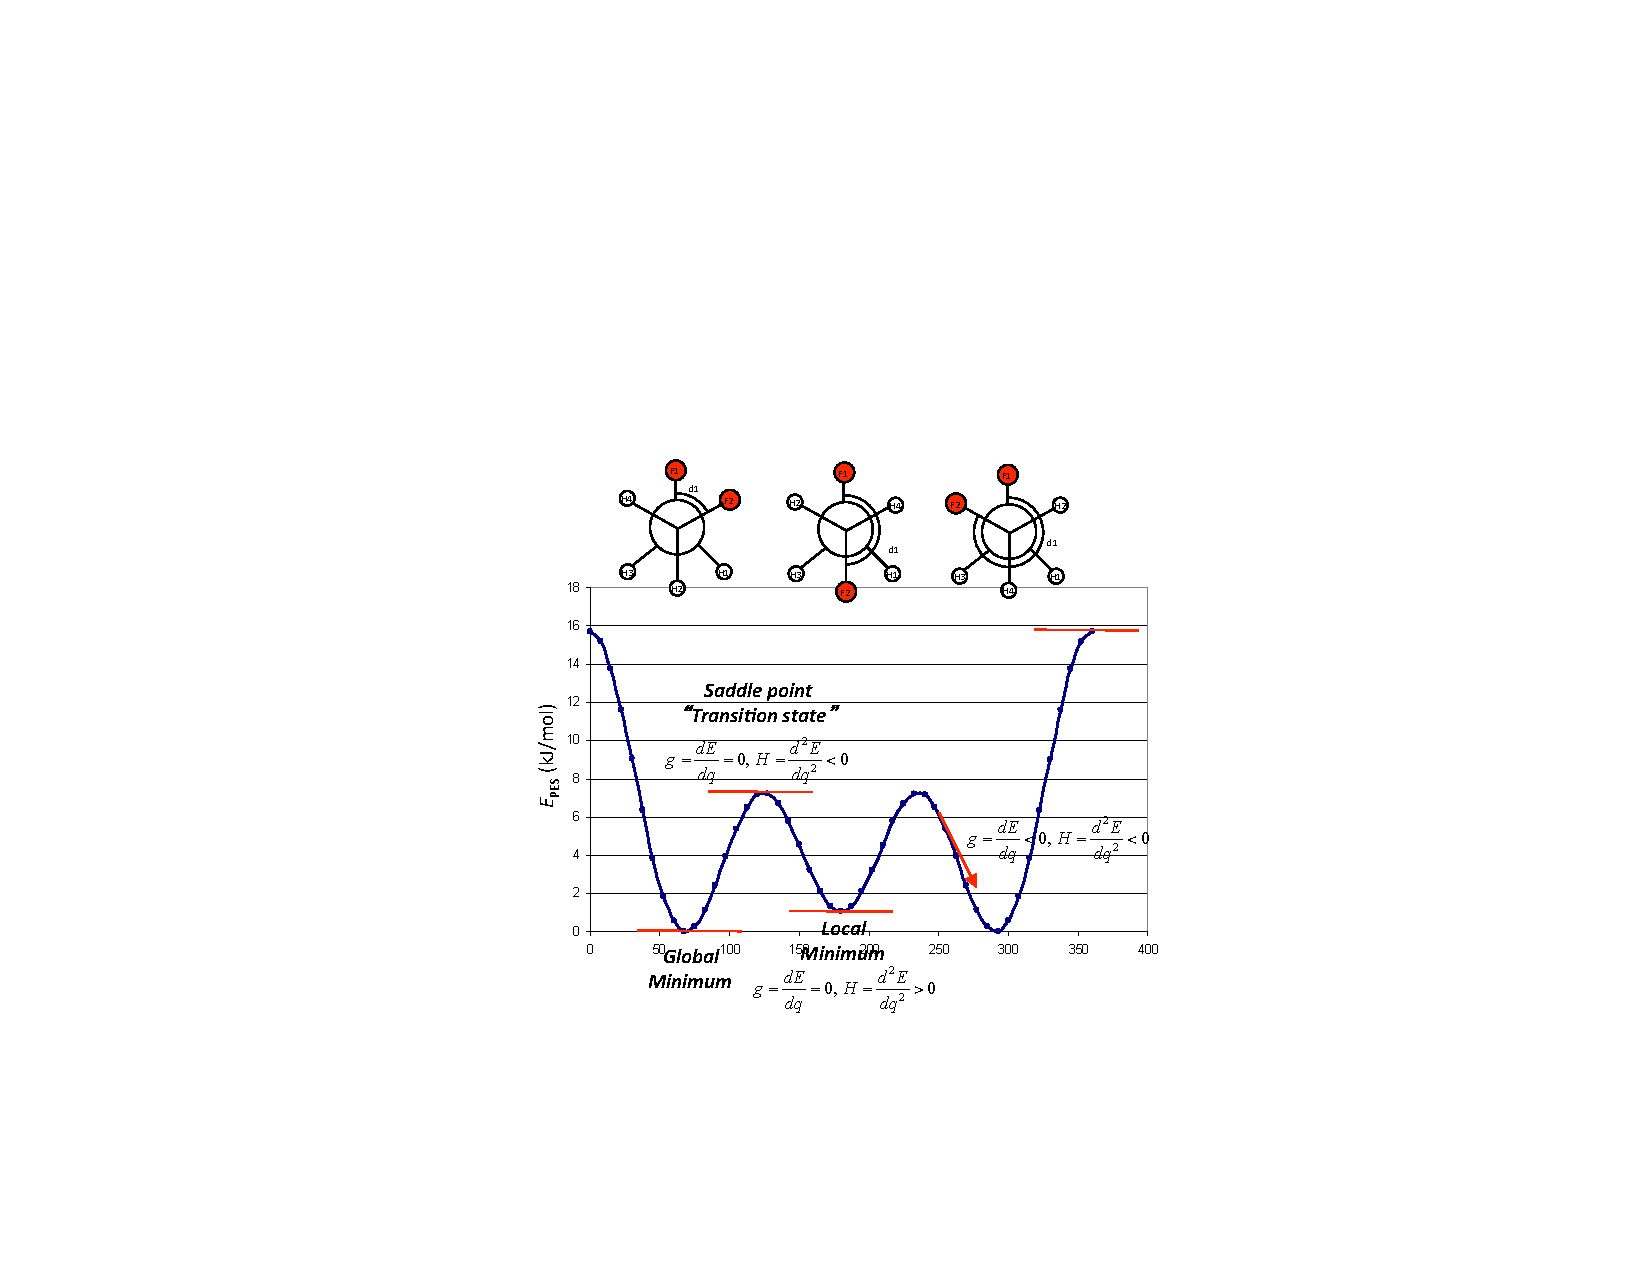
\includegraphics[width=0.75\textwidth]{./Images/PES.pdf}
\end{center}
\end{center}

\subsubsection{Gradients}
\label{sec:orgde48c24}

\subsubsection{Hessians}
\label{sec:orgd5a8d2a}

\subsubsection{Minima}
\label{sec:orgc7bee62}

\begin{itemize}
\item Local
\label{sec:orgc46940d}

\item Global
\label{sec:org1c6823f}
\end{itemize}

\subsubsection{Saddle points}
\label{sec:orge643a63}

\begin{itemize}
\item First-order
\label{sec:org686cd9c}

\item Higher order
\label{sec:org7282dc4}
\end{itemize}

\subsubsection{Minimum energy paths}
\label{sec:org3c050aa}

\subsection{Energy gradients and second derivatives}
\label{sec:orgfe9acbc}

\subsection{Optimization algorithms}
\label{sec:org7469c6f}
\subsubsection{Steepest descent}
\label{sec:org80b018a}

\subsubsection{Conjugate gradient}
\label{sec:org0040ccc}

\subsubsection{Quasi-Newton Raphson}
\label{sec:org63fc078}


\subsubsection{Direct inversion in the iterative subspace (DIIS)}
\label{sec:org747240b}
\subsubsection{Trudge}
\label{sec:org90f3bf3}
\subsubsection{Genetic algorithm}
\label{sec:orgeca0655}
\subsubsection{Convergence criteria}
\label{sec:org1d45a84}

\subsection{Geometry optimization algorithms}
\label{sec:orga772eeb}

\subsection{Efficient coordinate systems}
\label{sec:orgc4b8b4d}
\subsection{Performance of models}
\label{sec:orgb116ad6}
\subsection{Vibrational frequencies}
\label{sec:orgceacfea}
\subsection{Transition states}
\label{sec:org38c325a}
\subsection{Intrinsic reaction coordinates}
\label{sec:org441dfbe}
\newpage

\subsection{Molecular dynamics}
\label{sec:org2ffd368}

\section{\texttt{GAMESS} Cheat Sheet}
\label{sec:org0110403}
\subsection{Specifying electronic configuration}
\label{sec:orgddbe208}
\subsubsection{Closed shell (default)}
\label{sec:org0cbc1ef}
\begin{verbatim}
 $CONTRL RHFTYP=RHF MULT=1 $END
\end{verbatim}

\subsubsection{Open-shell (n = spin-multiplicity = \# unpaired electrons + 1)}
\label{sec:org395d6c6}
\begin{verbatim}
 $CONTRL RHFTYP=UHF MULT=n $END
\end{verbatim}
\subsection{Specifying electronic structure method}
\label{sec:org3127528}
\subsubsection{Hartree-Fock (default)}
\label{sec:orgba1b49c}
\subsubsection{DFT}
\label{sec:org54c0b53}
\begin{verbatim}
 $CONTRL DFTTYP=xxx $END
\end{verbatim}
\texttt{Gamess} supports \uline{many} DFT functionals.  See the \$DFT section of the manual for a full set.  Common DFT methods include:
\begin{center}
\begin{tabular}{ll}
\hline
method & xxx\\
\hline
Slater & Slater\\
Local density approx & SVN\\
Generalized gradient approx & PBE\\
Hybrid DFT & B3LYP\\
``Minnesota'' optimized & M06\\
 & M11\\
\hline
\end{tabular}
\end{center}
\subsubsection{Beyond Hartree-Fock}
\label{sec:org39986f8}
Many methods available.  See manual for full description.  Most common is second-order perturbation theory, ``MP2,'' :
\begin{verbatim}
 $CONTRL MPLEVL=2 $END
\end{verbatim}

If you want a very high quality number, have a big computer and time to wait, try ``coupled cluster,'':
\begin{verbatim}
 $CONTRL CCTYP=CCSD(T) $END
\end{verbatim}

\subsection{Specifying basis sets}
\label{sec:org2e924c6}
Gamess uses atom-centered basis functions.  A ``basis set'' is a set of such functions for many atoms, all constructed (hopefully) at a consistent level of accuracy. Many such basis sets exist and are coded into Gamess, and for the daring new basis sets can be input by hand.  Choice of basis set is always a compromise between accuracy and computational cost.  In general should always check sensitivity of property of interest to basis set.

Specified in \$BASIS group.  Some common choices, in increasing level of sophistication:

\begin{center}
\begin{tabular}{lll}
\hline
Name & Type & Flags\\
\hline
 & \textbf{Pople type} & \textbf{The most venerable and widely used}\\
STO-3G & Minimal & GBASIS=STO  NGAUSS = 3\\
3-21G & Split valence & GBASIS=N21  NGAUSS=3\\
6-31G(d) & Split valence polarized & GBASIS=N31 NGAUSS =6 NDFUNC=1\\
6-311+G(d,p) & Triple-split valence & GBASIS=N311 NGAUSS=6 NDFUNC=1 NPFUNC=1\\
 & polarized and augmented & DIFFSP=1\\
 &  & \\
 & \textbf{Polarization-consistent} & \textbf{Good for DFT}\\
PC0 & Minimal & GBASIS=PC0\\
PC1 & Split valence polarized & GBASIS=PC1\\
PC2 & Triple split double polarized & GBASIS=PC2\\
 &  & \\
 & \textbf{Correlation-consistent} & \textbf{Good for MP2 and beyond}\\
cc-pVDZ & Split valence polarized & GBASIS=CC2\\
cc-pVTZ & Triple split double polarized & GBASIS=CC3\\
 &  & \\
 & \textbf{Effective core potentials} & \textbf{Good for treating heavy atoms}\\
SBKJC & Split valence + core potential & GBASIS=SBKJC\\
Hay-Wadt & Split valence + core potential & GBASIS=HW\\
\hline
\end{tabular}
\end{center}

\subsection{Specifying geometry}
\label{sec:org8d63ea8}
Again \texttt{GAMESS} has a number of options, several of which are arcane and seldom used.  Most common are Cartesian and z-matrix.  Here I give examples ignoring any symmetry the molecule might have.
\subsubsection{Cartesian}
\label{sec:org16c8451}
Specify an atom name, atomic number, and cartesian positions in \AA{}.  Over-specified, so code will typically center and reorient.  Following is for gauche difluoroethane, \ce{FCH2CH2F}.
\begin{verbatim}
 $CONTRL COORD=CART $END
 $DATA
FCH2CH2F drag calculation
C1
C     6.0    -3.76764     0.33879     0.03727
C     6.0    -2.35246     0.34495     0.03689
F     9.0    -4.72277     0.58147    -1.18012
F     9.0    -1.59909    -0.68487    -0.83662
H     1.0    -4.04387     1.08375     0.75395
H     1.0    -3.92958    -0.71060     0.16941
H     1.0    -2.03786     0.18875     1.04760
H     1.0    -2.09983     1.28759    -0.40187
 $END
\end{verbatim}

\subsubsection{Z-matrix}
\label{sec:org853e56e}
Specify atom name, number of atom it is connected to, distance to that atom, number of atom it makes an angle with, value of the angle, number of the atom it makes a dihedral with, and value of the dihedral angle.  Values may be given directly or as variables, followed by list of variable specifications.  In \texttt{Gamess}, would specify z-matrix for \ce{FCH2CH2F} like this:
\begin{verbatim}
$CONTRL COORD=ZMT $END
$DATA
FCH2CH2F drag calculation
C1
C
C   1   r1
F   2   r2   1   A1
H   2   r3   1   A2   3   D1
H   2   r4   1   A3   3   D2
F   1   r2   2   A1   3   D3
H   1   r3   2   A2   6   D1
H   1   r4   2   A3   6   D2

r1=1.5386
r2=1.39462
r3=1.11456
r4=1.12
A1=109.54214
A2=111.
A3=110.
D1=120.
D2=-120.5
D3=50.
$END
\end{verbatim}
Particularly convenient when you'd like to ``scan'' over the value of some coordinate.  Variable can be applied to more than one independent coordinate, if the molecule has symmetry.  In general, though, variables should not be reused.

\subsection{Specify calculation type}
\label{sec:org72a6b8a}
Specified in \$CONTRL group by RUNTYP flag:

\begin{center}
\begin{tabular}{ll}
Calculation & RUNTYP=\\
\hline
Single-point energy & Energy\\
Single-point energy + force & Gradient\\
Geometry optimization & Optimize\\
Frequency calculation & Hessian\\
Transition state search & Sadpoint\\
Intrinisc reaction coordinate & IRC\\
\end{tabular}
\end{center}

Note too that specifying EXETYP=CHECK will check your input without actually running the job.
\subsection{Geometry optimization coordinate system}
\label{sec:org5c11345}
By default, \texttt{GAMESS} performs optimizations in Cartesian coordinates.

To use z-matrix coordinates, specify
\begin{verbatim}
 $CONTRL COORDS=ZMT NZVAR=xx $END
\end{verbatim}
where NZVAR = 3N-6.

To have \texttt{Gamess} automatically create a set of appropriate ``delocalized'' internal coordinates, specify
\begin{verbatim}
 $ZMAT DLC=.TRUE.  AUTO=.TRUE. $END
\end{verbatim}
\subsection{Performing a transition state search}
\label{sec:orgb538753}
Transition states are always more challenging to find than optimal geometries.  Always \texttt{at least} a three-step procedure:

\begin{enumerate}
\item Guess a transition state structure and compute Hessian matrix (RUNTYP = HESSIAN).  Check to be sure there is one imaginary mode approximating desired TS.
\item Perform the transition state search.  Must supply computed Hessian matrix, copied from .dat file, as \$HESS group.  Also should specify \$STATPT HESS=READ \$END.
\item Check the result!  Assuming the transition state search converges, run another frequency calculation to confirm that there is one and only one imaginary mode, and that it corresponds to desired TS.
\end{enumerate}

\section{Plane waves and core potentials}
\label{sec:org00ae442}

\subsection{Hydrogen atom in a box}
\label{sec:org18ad21c}

\subsection{Periodic boundary conditions}
\label{sec:org32b491c}

\subsection{Supercells - Cartesian and fractional coordinates}
\label{sec:org3b1ca58}

\subsection{Gaussian vs. Vasp}
\label{sec:org2aea883}

\subsection{Vasp POSCAR}
\label{sec:org5b20691}

\subsection{Vasp INCAR}
\label{sec:orgc0f298d}

\subsection{Core electron treatment}
\label{sec:org7990578}

\subsubsection{OPW}
\label{sec:orgc824762}

\subsubsection{PP}
\label{sec:org96f95c4}

\subsubsection{PAW}
\label{sec:orgc8e70e0}

\subsection{Comparing energies between calculations}
\label{sec:org79fe3bf}

\subsection{Wavefunctions and charge densities}
\label{sec:org28375c1}

\subsection{Exploring potential energy surfaces}
\label{sec:org0d31a2e}
\newpage
\section{Periodic electronic structure}
\label{sec:org0b8dde0}
\subsection{Isolated vs. periodic systems}
\label{sec:org6a681a1}
\subsection{Bloch's theorem and qualitative band structure}
\label{sec:org696a11c}
\subsection{Band folding}
\label{sec:org1e37dab}
\subsection{Multi-dimensional periodicity}
\label{sec:org8006ac4}
\subsection{Density of statues}
\label{sec:orge36b7c6}
\subsection{Bravais lattices}
\label{sec:org52727eb}
\subsection{Quantitative supercell calculations}
\label{sec:org819047e}
\subsection{Brillouin zone integration}
\label{sec:org6d19b2c}
\subsubsection{k-point sampling}
\label{sec:org6ce3c3b}
\subsubsection{Fermi smearing}
\label{sec:orge03065e}
\newpage
\section{Practical supercell calculations}
\label{sec:org96683b7}
\newpage
\section{Surfaces}
\label{sec:org374b28b}
\subsection{Surface planes}
\label{sec:org2f5af87}
\subsection{Slab models}
\label{sec:orgd87a117}
\subsection{Surface energy}
\label{sec:org6e1dbd5}
\subsection{Surface potentials and Fermi energies}
\label{sec:orga64ed7c}
\subsection{Surface adsorption}
\label{sec:orgca3e58d}
\subsection{Coverage-dependent adsorption}
\label{sec:org1f0ac6c}
\subsection{Reaction barriers}
\label{sec:orgebe4e21}

\newpage
\section{First-principles thermodynamics}
\label{sec:orgb01cb75}
\subsection{Connection Between QM and Thermodynamics}
\label{sec:org4d587bc}
We have focused to this point on the many approaches and details of calculating
the \emph{internal electronic energy} of a single molecule, that is, the energy
associated with taking infinitely separated constituent nuclei and electrons at
rest and forming a molecule:
\begin{equation}
2~\mathrm{H}^+ + 8~\mathrm{O}^{8+} + 10~\mathrm{e}^- \rightarrow
\mathrm{H_2O}\qquad E^\mathrm{elec}
\end{equation}
\(E^\mathrm{elec}\) is typically calculated within the Born-Oppenheimer
approximation, i.e.$\backslash$ within the approximation that the nuclei are fixed in space
at the minimum energy configuration.  Even at 0\textasciitilde{}K, by quantum mechanics the
atoms must vibrate about this minimum, and this intrinsic vibration imparts a
\emph{zero-point vibrational energy} (ZPVE) to the molecule, and the 0\textasciitilde{}K
internal energy of a molecule is thus:
\begin{equation}
  E^0=E^\mathrm{elec} + ZPVE
\end{equation}
ZPVE can be calculated reliably within the harmonic approximation, according to
\begin{equation}
  \mathrm{ZPVE}=\frac{1}{2}h\sum_{i=1}^{3n-6}\nu_i
\end{equation}
where \(\nu_i\) are the harmonic vibrational frequencies, obtained from a
vibrational frequency analysis.  \(E^0\) is the minimum physically meaninfful
energy of the molecule.

Energy can be deposited in a molecule in many other ways as well, e.g.$\backslash$ as
translational and rotational kinetic energy, in excited vibrational modes, in
the interaction of a molecule with an external electric or magnetic or
gravitational field, or \ldots{}.  If we assume that the energy in these various
degrees of freedom are separable, we can write:
\begin{equation}
  E_i=E^0+E^\mathrm{trans}+E^\mathrm{rot}+E^\mathrm{vib} +E^\mathrm{elec*}+E^\mathrm{ext}
\end{equation}
To fully describe microscopic energetic state of a molecule, would have to
specify all of these.

Typically, though, we are more interested in the collective properties of many
molecules at equilibrium, like the internal energy \(U\) or enthalpy \(H\) or Gibbs
energy \(G\), under some external constraints like temperature \(T\) or volu
me \(V\).  These thermodynamic quantities are averages over the energy states of
an \emph{ensemble} of molecules.  The way this averaging is performed is the
realm of \emph{statistical thermodynamics}.

Most important for us will be the \emph{canonical ensemble}, in which the free
variables are the number of molecules \(N\), the total volume \(V\), and the
temperature \(T\).  Offer without proof, in the canonical ensemble the
probability for a molecule to be in some energy state \(E_i\) above \(E^0\) is
given by the Boltzmann factor,
\begin{equation}
  P(E_i) \propto e^{-E_i\beta}=e^{-E_i/k_BT},\qquad\beta=1/k_BT
\end{equation}
Defines an exponentially decaying probability function for a state to be
occupied at some temperature.  In a sense, \emph{temperature} is the property of
a system following this distribution.
\begin{figure}[h]
  \centering
  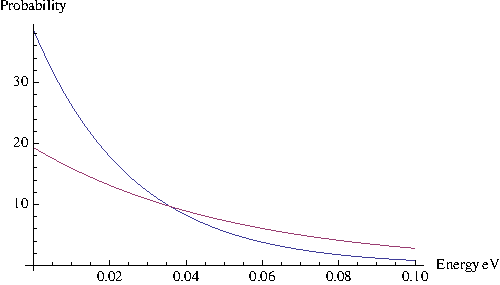
\includegraphics{./Images/boltzmann}
  \caption{Boltzmann distribution at two different temperatures}
  \label{fig:boltzmann}
\end{figure}

\subsubsection{Averages and partition functions}
\label{sec:org1f52832}
Let's use this to calculate the internal energy \(U\) of a molecule at some
temperature.
\begin{equation}
  U(T)=\frac{\sum_iE_iP(E_i)}{\sum_iP(E_i)}
\end{equation}
where the denominator ensures that the probability is normalized.
\begin{eqnarray}
  U(T) & =& \frac{\sum_iE_i e^{-E_i\beta}}{\sum_ie^{-E_i\beta}} \\
  & = & \frac{\frac{\partial}{\partial\beta}\sum_ie^{-E_i\beta}}{\sum_ie^{-E_i
      \beta}}\\
& = & -\frac{\partial \ln \sum_i e^{-E_i\beta}}{\partial \beta}
\end{eqnarray}
The sum over energy states is evidently a special quantity, called the
partition function:
\begin{equation}
  q=\sum_ie^{-E_i\beta}
\end{equation}
All thermodynamic quantities can be written in terms of the partition function!

\subsubsection{Harmonic oscillator example}
\label{sec:org9656656}
Harmonic oscillator is a reasonable model of a molecular vibration.  Energy
spectrum given by
\begin{equation}
  E_v=(v+1/2)h\nu,\qquad v=0,1,2,...
\end{equation}
Let's define the energy qunatum \(h\nu=\epsilon_0\) and reset the energy scale so
that zero is at \(1/2 h\nu\):
\begin{eqnarray}
  E_v & = & v\epsilon_0,\qquad v=0,1,2,... \\
q(T) & = &\sum_{v=0}^\infty e^{-v\epsilon_0\beta} \\
 & = & \frac{1}{1-e^{-\epsilon_0\beta}}
\end{eqnarray}
where we take advantage of the fact that the sum is a geometric series to
evaluate it in closed form.

Plot partition function vs \(T\), increasing function.

\noindent Internal energy:
\begin{eqnarray}
  U(T) &=&-\frac{\partial \ln q}{\partial \beta}\\
   & = & \frac{\epsilon_0}{e^{\epsilon_0\beta}-1}
\end{eqnarray}

\noindent Heat capacity:

\noindent Entropy

\subsection{Molecular Ideal Gas}
\label{sec:org09e4921}
Nice example above for a simple model.  To get thermodynamics of an ideal gas,
in principle need to sum over all the types of energy states (translational,
rotational, vibrational, \ldots{}) of every molecule.  Seemingly impossible task.
One simplification is if we can write energy as sum of energies of individual
elements (molecules) of system:
\begin{align}
  E_j&=\epsilon_j(1)+\epsilon_j(2) + ... + \epsilon_j(N) \\
  Q(N,V,T) &= \sum_j e^{-E_j\beta} \\
  &=\sum_je^{-(\epsilon_j(1)+\epsilon_j(2) + ... + \epsilon_j(N))\beta}
\end{align}
\emph{If} molecules/elements of system can be distinguished from each
        other (like atoms in a fixed lattice), expression can be factored:
  \begin{align}
    Q(N,V,T)&=\left ( \sum_j e^{-\epsilon_j(1)\beta}\right )\cdots \left ( \sum_j
      e^{-\epsilon_j(N)\beta}\right ) \\
  &= q(1)\cdots q(N) \\
  \text{Assuming all the elements are the same:}\\
  &= q^N
\end{align}
\emph{If not} distinguishable (like molecules in a liquid or gas, or
      electrons in a solid), problem is difficult, because identical
      arrangements of energy amongst elements should only be counted once.
      Approximate solution, good almost all the time:
\begin{equation}
  Q(N,V,T)=q^N/N!
\end{equation}
Sidebar: ``Correct'' factoring depends on whether individual elements
     are fermions or bosons, leads to funny things like superconductivity and
     superfluidity.

This \(q(V,T)\) is the \emph{molecular partition function}, and is calculated by
summing over the individual energy states of a single molecule (starting at \(E_0\)).

Further simplified by factoring into contributions from various (\(3N\)) molecular
degrees of freedom:
\begin{eqnarray}
  q(V,T)&=&\left(\sum_\mathrm{trans}
    e^{-e_\mathrm{trans}\beta}\right) \left(\sum_\mathrm{rot}
  e^{-e_\mathrm{rot}\beta}\right) \left( \sum_\mathrm{vib}
  e^{-e_\mathrm{vib}\beta} \right) \left( \sum_\mathrm{elec}
  e^{-e_\mathrm{elec}\beta}\right) \\
&=& q_\mathrm{trans}q_\mathrm{rot}q_\mathrm{vib}q_\mathrm{elec} \\
U & = & E_0 + U_\mathrm{trans}+U_\mathrm{rot}+U_\mathrm{vib}+U_\mathrm{elec}
\end{eqnarray}
Similarly for other thermodynamic quantities, for example,
\begin{equation}
  C_v=\left(\frac{\partial U}{\partial T}\right)_V = C_{v,\mathrm{trans}}+C_{v,\mathrm{rot}}+C_{v,\mathrm{vib}}+C_{v,\mathrm{elec}}
\end{equation}
Thermodynamic quantities are sums of contributions from indvidual degrees of
freedom.

Have to somehow \emph{model} these motions and have to use our quantum
mechanical results to parameterize the models.

\subsubsection{Translational partition function}
\label{sec:orgc05730b}
Need a model molecules freely translating about in a box.  How about the
\emph{particle in a box}?
\begin{equation}
  E_n=\frac{n^2\pi^2\hbar^2}{2 m L^2},~~~~~n=1,2,3,...
\end{equation}
Have to construct partition function for one molecule.  For gas molecules at
normal conditions, energy spacing is tiny.  Spare the details, but find that
\(q_\mathrm{trans}\) can be written in terms of a \emph{thermal wavelength}
\(\Lambda\):
\begin{eqnarray}
  \Lambda=\frac{h}{\sqrt{2\pi m k_B T}} \\
q_\mathrm{trans}=\frac{V^\circ}{\Lambda^3}
\end{eqnarray}
\(\Lambda\) depends only a molecule mass (that's easy!) and is of the order the
box dimensions at which quantization is evident.  Typically a tiny number
(e.g. \$1.7\texttimes{} 10\(^{\text{-11}}\)\$\textasciitilde{}m for Ar in a 1 liter volume at 298 K.
\(q_\mathrm{trans}\) is, on the other hand, enormous: lots of translational
freedom.  \(V^\circ\) defines the standard state volume.

Given this, can find all translational contributions to thermodynamics.
\(S_\mathrm{trans}\) gives the Sackur-Tetrode equation, the absolute entropy of a
monatomic gas:


\subsubsection{Rotational partition function}
\label{sec:orgec4144b}
Model molecule as a rigidly rotating body.  Body has three orthogonal moments
of inertia \(I\) determined by the molecular structure.

\subsubsection{Vibrational partition function}
\label{sec:orgb3fb7e3}
See harmonic oscillator above

\subsubsection{Electronic partition function}
\label{sec:org4398e6a}
Governed by Fermi-Dirac distribution
Electronic degeneracy


\subsection{CO T-dependent thermo example}
\label{sec:orgd65b685}
\newpage
\section{Implicit solvation}
\label{sec:org891f6d4}
\section{Density functional theory}
\label{sec:org3dedbb9}
\subsection{Electron density \(\rho\) as fundamental quantity}
\label{sec:orgd1ea882}
\subsection{Thomas-Fermi-Dirac model}
\label{sec:org8eed05b}
\subsection{Hartree-Fock-Slater model}
\label{sec:org13a7be5}
\subsection{Hohenberg-Kohn theorems}
\label{sec:orgbaa990e}
\subsection{Kohn-Sham construction}
\label{sec:org3549178}
\subsection{Exchange-correlation functionals}
\label{sec:orgdb1a256}
So Kohn et al. showed that the DFT approach is theoretically well-grounded and
provided one way to practically apply it. Promise is that if we can find an
approximation to the (unknown) true \(v_\text{xc}\) with the right balance of simplicity
and accuracy, we will have one sweet theory. Has to incorporate both exchange,
like Slater tried to do, and correlation.

How to proceed? Lots of approaches, and jargon here is at least as bad as in
wavefunction-based methods. Perdew 2006 describes the ``Jacob's ladder'' of
approximations:
\subsubsection{LDA}
\label{sec:orgae0111b}
One well-defined limit is the homogeneous electron gas, and this is the usual
starting point for modern approximate DFT methods. Assume exchange and
correlation potentials at any given point depend only on the value of \(\rho\) there
(or spin-up and spin-down \(\rho\), if spin-polarized). We know from Slater and
Dirac's work what the exchange potential is for this system.

It is possible to determine numerically the correlation energy for a given
density from quantum Monte Carlo calculations. Ceperley and Alder (PRL 1980,
45, 566) did this to very high accuracy, and others (Vosko, Wilk, and Nusair,
``VWN'', and Perdew and Wang, ``PW'') fit these numerical results to analytical
models in \(\rho\). This combination of local exchange and correlation defines the LDA
model.

LDA offers modest improvement over HFS for molecules. ``Homogeneous''
approximation pretty severe for an atom or molecule. Nonetheless, works
surprisingly well for structures and charge distributions, but has problems in
calculating accurate bond energies, typically overbinding. Also tends to
underestimate the HOMO-LUMO gap in molecules and analogous band gap in solids.

\subsubsection{GGA}
\label{sec:org58bd482}

\subsubsection{Meta-GGA}
\label{sec:orge7410ed}

\subsubsection{Hyper GGA and hybrid functionals}
\label{sec:orgb6b29bb}

\begin{itemize}
\item ``Screened'' exchange
\label{sec:orgac419e6}
\end{itemize}

\subsubsection{Beyond hyper GGA}
\label{sec:org355f3c2}

\subsection{Implementations}
\label{sec:org3c09386}

\subsection{Performance}
\label{sec:org3becf3d}
\newpage
\newpage
\section{Electron correlation methods}
\label{sec:org8a43fc4}
\newpage
\end{document}